\documentclass[handout, table,svgnames,hyperref={pdfpagemode=FullScreen}]{beamer}
\usepackage[utf8]{inputenc}
\usepackage{graphicx}
\usepackage{color, colortbl}
%\usepackage[table]{xcolor}
%\usepackage[svgnames]{xcolor}
\usepackage{listings}
%\usetheme{Frankfurt}
\usetheme{Boadilla}
%-------------------TITRE------------------------%
\title{\textsc{Formation \\ Langage de programmation - R}}
%---------------Date à remplir ou commenter pour date du jour-------------%
%\institute{BiRD - Inserm}
\date{26 septembre 2013}
\logo{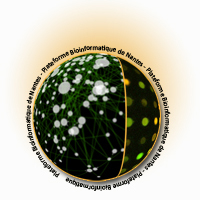
\includegraphics[height=10mm]{image/logo.jpg}}
%--------Rédacteur------------%
\author{\textsc{Édouard Hirchaud \\ Floriane Simonet}} 

\usepackage{pslatex}
\usepackage{tikz}

\setbeamertemplate{blocks}[rounded]%
[shadow=true]

	\newcolumntype{g}{>{\columncolor{blue!10}}c}
\newcommand{\CodeSymbol}[1]{\bfseries\textcolor{DarkRed}{#1}}
\lstset{
language=R,
basicstyle=\ttfamily\scriptsize,
commentstyle=\ttfamily\color{DarkBlue},
%numbers=left,
numberstyle=false,
%stepnumber=1,
%numbersep=5pt,
backgroundcolor=\color{white},
showspaces=false,
showstringspaces=false,
showtabs=false,
frame=single,
tabsize=2,
captionpos=b,
%breaklines=true,
breakatwhitespace=false,
%title=\lstname,
escapeinside={},
keywordstyle=\bfseries\color{DarkGreen},
morekeywords={},
literate={é}{{\'e}}1
	{è}{{\`e}}1
		{ê}{{\^e}}1
		{à}{{\`a}}1
		{ç}{{\c{c}}}1
		{(}{{\CodeSymbol{(}}}1
		{)}{{\CodeSymbol{)}}}1
%		{\[}{{\CodeSymbol{\[}}}1
%		{\]}{{\CodeSymbol{\]}}}1
}


\newcommand{\grille}{
\begin{tikzpicture}[overlay,remember picture]
	\begin{scope}[shift={(current page.south west)}]
		\draw[gray!50] (0,0) grid[step=2mm] (current page.north east);
		\draw[red!50] (0,0) grid[step=1cm] (current page.north east);
		\draw (0.2,1) node {1};
     \draw (0.2,2) node {2};
     \draw (0.2,3) node {3};
     \draw (0.2,4) node {4};
     \draw (0.2,5) node {5};
     \draw (0.2,6) node {6};
     \draw (0.2,7) node {7};
     \draw (0.2,8) node {8};
     \draw (0.2,9) node {9};
     \draw (1,0.5) node {1};
     \draw (2,0.5) node {2};
     \draw (3,0.5) node {3};
     \draw (4,0.5) node {4};
     \draw (5,0.5) node {5};
     \draw (6,0.5) node {6};
     \draw (7,0.5) node {7};
     \draw (8,0.5) node {8};
     \draw (9,0.5) node {9};
     \draw (10,0.5) node {10};
     \draw (11,0.5) node {11};
     \draw (12,0.5) node {12};
\end{scope}
\end{tikzpicture}
}


%Definition de couleur en RGB
%\definecolor{LightRed}{RGB}{255,204,204}
%\definecolor{LightGreen}{RGB}{153,255,153}

\begin{document}

\begin{frame}
	\maketitle
%	\titlepage
\end{frame}
	

\section*{Sommaire}
\begin{frame}{Sommaire}
	%\tiny \tableofcontents[hideothersubsections]
	\small \tableofcontents
\end{frame}

\section{Notions informatiques}

\subsection{Systèmes d'exploitation}
\begin{frame}
	\frametitle{Les systèmes d'exploitation : OS (Operating System)}
	\begin{figure}
		
\includegraphics[scale=0.55]{image/OSimage.png}
	\end{figure}
\end{frame}

\subsection{Les applications}
\begin{frame}
	\setbeamercovered{dynamic}
	\frametitle{Les applications : logiciels, programmes}
	\begin{figure}[h]
		\begin{center}
		  
\includegraphics[scale=0.45]{image/software.png}
		\end{center}
	\end{figure}
\end{frame}


\subsection{Chemins et fichiers}
\begin{frame}
	\frametitle{Arborescence}
	\begin{block}{Appellation}
		\begin{itemize}
			\item Fichiers : Données numériques
			\item Directory = Répertoire = Dossier : contient des fichiers.
		\end{itemize}
	\end{block}
	\begin{columns}
		\begin{column}[c]{5cm}
			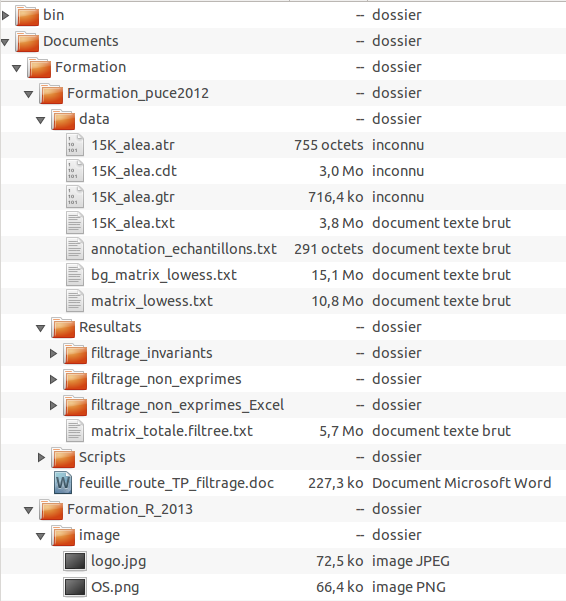
\includegraphics[scale=0.25]{image/ArboUbuntu.png}
		\end{column}
			\begin{column}[c]{5cm}
				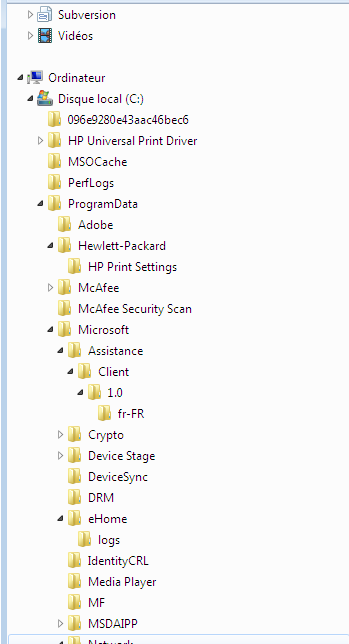
\includegraphics[scale=0.25]{image/ArboWin.png}
			\end{column}
		\end{columns}
\end{frame}

\begin{frame}
		\frametitle{Schématisation}
		\begin{center}
			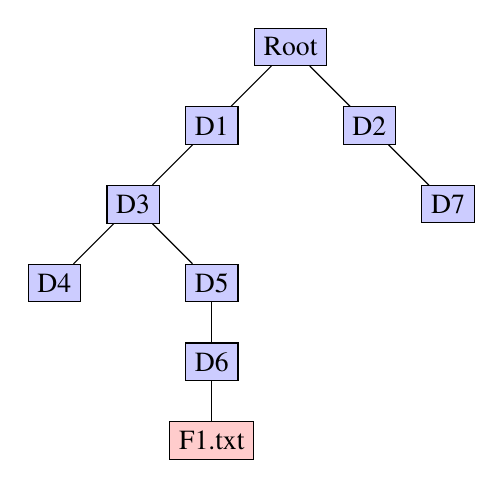
\begin{tikzpicture}[directory/.style={rectangle,draw,fill=blue!20},
				file/.style={rectangle,draw,fill=red!20}]
	\node[directory] (R) at  (0,0) {Root};
	\node[directory] (D1) at (-1,-1) {D1};
	\node[directory] (D2) at (1,-1) {D2};
	\node[directory] (D3) at (-2,-2) {D3};
	\node[directory] (D7) at (2,-2) {D7};
	\node[directory] (D4) at (-3,-3) {D4};
	\node[directory] (D5) at (-1,-3) {D5};
	\node[directory] (D6) at (-1,-4) {D6};
	\node[file] (F1) at (-1,-5) {F1.txt};
	\draw[-] (R) -- (D1);
	\draw[-] (R) -- (D2);
	\draw[-] (D1) -- (D3);
	\draw[-] (D3) -- (D4);
	\draw[-] (D3) -- (D5);
	\draw[-] (D5) -- (D6);
	\draw[-] (D6) -- (F1);
	\draw[-] (D2) -- (D7);
\end{tikzpicture}


		\end{center}
\end{frame}	

\begin{frame}
		\frametitle{La navigation}
		\begin{block}{Deux types de navigation}
			\begin{itemize}
				\item Chemin absolu
				\item Chemin relatif
			\end{itemize}
		\end{block}
		\begin{block}{Symboles utilisés dans la navigation}
			\begin{itemize}
				\item La racine : Windows une lettre, Linux et mac, symbole / 
				\item Séparateur de répertoire : Windows  \textbackslash, Linux et mac  /
				\item Le Répertoire courant : . (point)
				\item Le Répertoire parent : .. (deux points)
			\end{itemize}
		\end{block}
\end{frame}

\begin{frame}
		\frametitle{Formalisation : Chemin absolu}
		\begin{columns}
			\begin{column}[l]{5cm}
				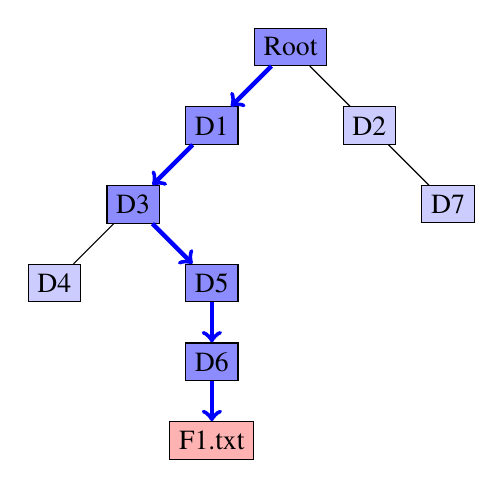
\begin{tikzpicture}[directory/.style={rectangle,draw,fill=blue!20},
					directoryA/.style={rectangle,draw,fill=blue!45},	
	file/.style={rectangle,draw,fill=red!30}]
	\node[directoryA] (R) at  (0,0) {Root};
	\node[directoryA] (D1) at (-1,-1) {D1};
	\node[directory] (D2) at (1,-1) {D2};
	\node[directoryA] (D3) at (-2,-2) {D3};
	\node[directory] (D7) at (2,-2) {D7};
	\node[directory] (D4) at (-3,-3) {D4};
	\node[directoryA] (D5) at (-1,-3) {D5};
	\node[directoryA] (D6) at (-1,-4) {D6};
	\node[file] (F1) at (-1,-5) {F1.txt};
	\draw[->, color=blue, ultra thick] (R) -- (D1);
	\draw[-] (R) -- (D2);
	\draw[->, color=blue ,ultra thick] (D1) -- (D3);
	\draw[-] (D3) -- (D4);
	\draw[->, color=blue,ultra thick] (D3) -- (D5);
	\draw[->, color=blue,ultra thick] (D5) -- (D6);
	\draw[->,color=blue,ultra thick] (D6) -- (F1);
	\draw[-] (D2) -- (D7);
\end{tikzpicture}


			\end{column}
			\begin{column}[r]{5cm}
				\begin{block}{Chemin absolu}
					\begin{itemize}
						\item À partir de la racine 
						\item Root/D1/D3/D5/D6/F1.txt
					\end{itemize}
				\end{block}
			\end{column}
		\end{columns}
\end{frame}

\begin{frame}
		\frametitle{Formalisation : Chemin relatif exemple 1}
		\begin{columns}
			\begin{column}[l]{5cm}
				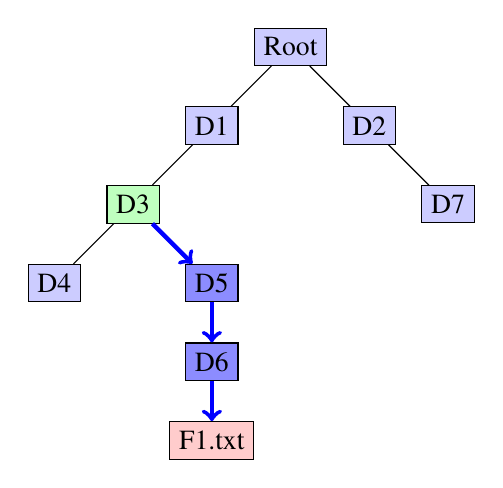
\begin{tikzpicture}[directory/.style={rectangle,draw,fill=blue!20},
				file/.style = {rectangle, draw, fill=red!20},
				directoryC/.style={rectangle, draw, fill=green!25},
				directoryR/.style={rectangle, draw, fill=blue!45}]
	\node[directory] (R) at  (0,0) {Root};
	\node[directory] (D1) at (-1,-1) {D1};
	\node[directory] (D2) at (1,-1) {D2};
	\node[directoryC] (D3) at (-2,-2) {D3};
	\node[directory] (D7) at (2,-2) {D7};
	\node[directory] (D4) at (-3,-3) {D4};
	\node[directoryR] (D5) at (-1,-3) {D5};
	\node[directoryR] (D6) at (-1,-4) {D6};
	\node[file] (F1) at (-1,-5) {F1.txt};
	\draw[-] (R) -- (D1);
	\draw[-] (R) -- (D2);
	\draw[-] (D1) -- (D3);
	\draw[-,] (D3) -- (D4);
	\draw[->, color = blue, ultra thick] (D3) -- (D5);
	\draw[->, color = blue, ultra thick] (D5) -- (D6);
	\draw[->, color = blue, ultra thick] (D6) -- (F1);
	\draw[-] (D2) -- (D7);
\end{tikzpicture}


			\end{column}
			\begin{column}[r]{5cm}
				\begin{block}{Chemin relatif}
					\begin{itemize}
						\item D5/D6/F1.txt
					\end{itemize}
				\end{block}
			\end{column}
		\end{columns}
\end{frame}

\begin{frame}
		\frametitle{Formalisation : Chemin relatif exemple 2}
		\begin{columns}
			\begin{column}[l]{5cm}
				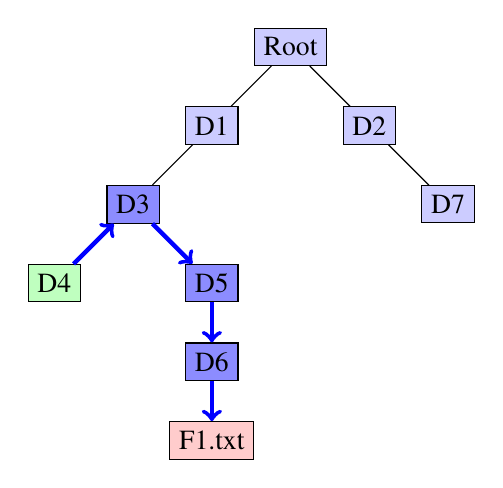
\begin{tikzpicture}[directory/.style={rectangle,draw,fill=blue!20},
				file/.style = {rectangle, draw, fill=red!20},
				directoryC/.style={rectangle, draw, fill=green!25},
				directoryR/.style={rectangle, draw, fill=blue!45}]
	\node[directory] (R) at  (0,0) {Root};
	\node[directory] (D1) at (-1,-1) {D1};
	\node[directory] (D2) at (1,-1) {D2};
	\node[directoryR] (D3) at (-2,-2) {D3};
	\node[directory] (D7) at (2,-2) {D7};
	\node[directoryC] (D4) at (-3,-3) {D4};
	\node[directoryR] (D5) at (-1,-3) {D5};
	\node[directoryR] (D6) at (-1,-4) {D6};
	\node[file] (F1) at (-1,-5) {F1.txt};
	\draw[-] (R) -- (D1);
	\draw[-] (R) -- (D2);
	\draw[-] (D1) -- (D3);
	\draw[<-, color = blue, ultra thick] (D3) -- (D4);
	\draw[->, color = blue, ultra thick] (D3) -- (D5);
	\draw[->, color = blue, ultra thick] (D5) -- (D6);
	\draw[->, color = blue, ultra thick] (D6) -- (F1);
	\draw[-] (D2) -- (D7);
\end{tikzpicture}


			\end{column}
			\begin{column}[r]{5cm}
				\begin{block}{Chemin relatif}
					\begin{itemize}
						\item ../D5/D6/F1.txt
					\end{itemize}
				\end{block}
			\end{column}
		\end{columns}
\end{frame}

\subsection{Types de mémoires}
\begin{frame}
		\frametitle{Les mémoires}
		\begin{columns}
		  \begin{column}[c]{5cm}
		    \begin{figure}[h]
		      \begin{center}
			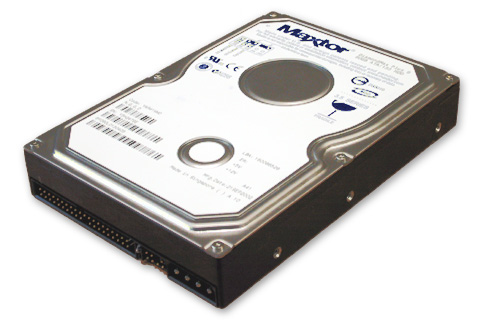
\includegraphics[scale=0.35]{image/hdd.jpg}
		      \end{center}
		    \end{figure}
		  \end{column}
		  \begin{column}[c]{5cm}
		    \begin{figure}[h]
		      \begin{center}
			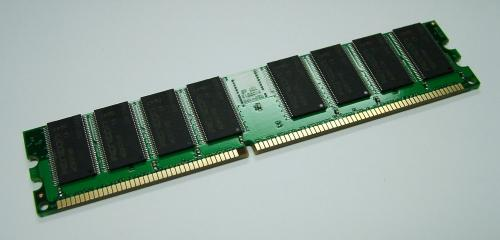
\includegraphics[scale=0.40]{image/memory_chip.jpg}
		      \end{center}
		    \end{figure}
		  \end{column}
		\end{columns}
\end{frame}

 \subsection{Synthèse}
\begin{frame}
	  \setbeamercovered{dynamic}
	  \frametitle{Synthèse}
	  \begin{figure}[h]
	    \begin{center}
	      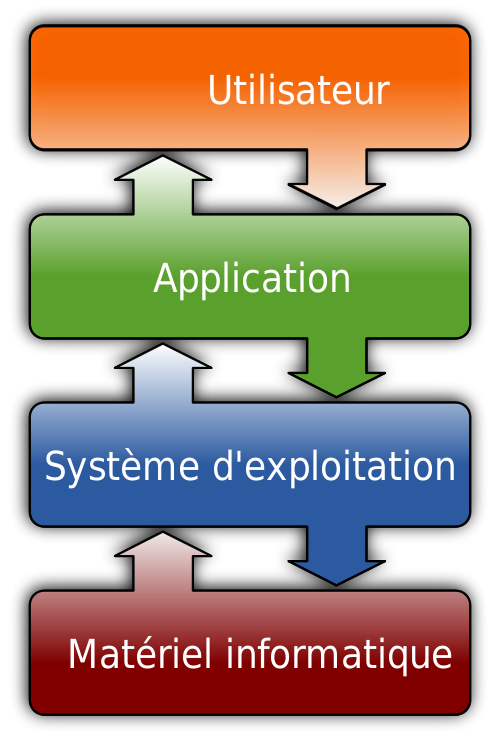
\includegraphics[scale=0.25]{image/OS.png}
	    \end{center}
	  \end{figure}
\end{frame}




\section{R}
\subsection{Aperçu}

\begin{frame}
	\frametitle{R : Aperçu}
	\begin{center}
		\begin{block}{}
			\begin{itemize}
				\item Créé par Ross Ihaka et Robert Gentleman (1996)
				\item C'est un logiciel libre et gratuit
				\item Disponible sur les systèmes d'exploitation les plus utilisés
				\item Utilisé dans de nombreux domaines dont la bioanalyse.
			\end{itemize}
		\end{block}
	\end{center}
\end{frame}

\subsection{Objectif du TP}
\begin{frame}
	\frametitle{Objectif du TP}
	\setbeamercovered{dynamic}
		
	\begin{itemize}[<+->]
		\item {Assimiler le vocabulaire }
		\item {Se servir de R comme d'une calculatrice}
		\item {Écrire et modifier des lignes de commande}
		\item {Utiliser un script déjà écrit}
		\item {Savoir où trouver de l'aide (documentation)}
		\item {Utiliser un éditeur convivial (RStudio)}%
	\end{itemize}
\end{frame}

\subsection{Comparaison Excel R}
\begin{frame}
	\frametitle{Comparaison Excel R}
%	\setbeamercovered{dynamic}
	\begin{center}
%		\setlength\doublerulesep{3pt}
%		\doublerulesepcolor{blue!15}
{\rowcolors[]{1}{blue!20}{blue!10}
	\begin{tabular}[h]{cc}
		\hline
		\textbf{Excel} &  \textbf{R} \pause\\
		\hline 
		
		Cellule & Élément simple \\
		Plage de données & data.frame matrix, list, vector \pause\\
		\hline
		Valeur & Valeur (value) \\
		Format & Type \pause\\
		\hline
		Fonction & Fonction \\
		Macro & Script \\
		\hline
	\end{tabular}}
	\end{center}
\end{frame}
\subsection{Les objets}
\begin{frame}
	\setbeamercovered{dynamic}
	\frametitle{Les Objets}
	\begin{exampleblock}{Deux types d'objets à retenir}
	\begin{itemize}
		\item Les objets de données
		\item Les fonctions
	\end{itemize}
	\end{exampleblock}
\end{frame}
\begin{frame}
	\frametitle{Les Objets de données}
	\setbeamercovered{dynamic}
	\begin{itemize}
		\item Un nom : que l'on appelle  variable
		\item Valeur(s)
		\item Les valeurs ont un type : 
			\begin{itemize}
				\item numérique : 1,2, 3.14
				\item chaîne de caractères : A,B gènes
				\item logique : TRUE/FALSE
			\end{itemize}
	\end{itemize}
	Les objets sont temporaires, ils sont stockés dans la mémoire vive de l'ordinateur. Il faudra donc les sauvegarder.
\end{frame}

\begin{frame}
	\frametitle{Catégories de données}
	\setbeamercovered{dynamic}
%	\begin{center}
		\begin{itemize}[<+->]
			\item vector $\Rightarrow$ vecteur (type homogène)
			\item matrix $\Rightarrow$ matrice (type homogène)
			\item data.frame $\Rightarrow$ tableau de données (type hétérogène)
			\item factor $\Rightarrow$ classe de paramètres qualitatifs (type homogène)
			\item list $\Rightarrow$ liste( type hétérogène)
		\end{itemize}
%	\end{center}
\end{frame}
\begin{frame}[fragile]
	%\setbeamercovered{dynamic}
	\frametitle{Création d'objets}

	\lstinputlisting{code/myVector.R}


\end{frame}
\begin{frame}
	\setbeamercovered{dynamic}
	\frametitle{Accéder aux valeurs}
	\begin{exampleblock}{Notion d'indices ou index}
		\begin{itemize}
			\item Les indices sont entourés de crochets 
			\item Il s'agit de la position d'une valeur
			\item Pour les vecteurs, simple indice. $[i]$
			\item Pour les data.frame et matrice, double indice, $[Ligne, Colone]$
		\end{itemize}
	\end{exampleblock}
	
\end{frame}
\begin{frame}[fragile]
	\frametitle{Vecteur}
	\begin{lstlisting}
	monVecNum <- c(500 , 452, 8)
	element3 <- monVecNum[3]
	\end{lstlisting}
	\begin{table}[ht]
		\begin{tabular}{l|c|c|g|}
			\emph{Indices} & $[1]$ & $[2]$ & $[3]$ \\
			 \hline
			 \emph{Valeurs} & 500 & 452 & 8 \\
		\end{tabular}
	\end{table}

\end{frame}
\begin{frame}[fragile]
	\frametitle{Matrices}
	\setbeamercovered{dynamic}
	\begin{lstlisting}
	 maMatrice <- matrix(1:15, ncol=5)
	 maLigne2 <- maMatrice[2, ]
	 maColone3 <- maMatrice[, 3]
	 elementL2C3<- maMatrice[2,3]
	\end{lstlisting}
	\begin{table}[ht]
	%	{\rowcolors[]{1}{gray!20}{gray!10}
		\begin{tabular}{|c|c|c|g|c|c|}
			\hline
			 & $[, 1]$ & $[, 2]$ & $[, 3]$ & $[, 4]$  & $[, 5]$ \\
			\hline
			$[1, ]$ & 1 & 2 & 3 & 4 & 5 \\
			\hline
			\rowcolor{blue!20}
			$[2, ]$ & 6 & 7 & \cellcolor{blue!40}8 & 9 & 10  \\
			\hline
			$[3, ]$ & 11 & 12 & 13 & 14 & 15  \\
			\hline
		\end{tabular}
	\end{table}
\end{frame}
\begin{frame}
	\frametitle{Data Frame}
	\begin{center}
	\lstinputlisting{code/dataFrame.R}
	\begin{tabular}{|c|c|g|}
		\hline
		& \textbf{Ech} & \textbf{Type} \\
		\hline
		$[1,]$ &1 & WT \\ 
		\hline
		$[2,]$ &2 & WT\\ 
		\hline
		$[3,]$ &3 & MUT1\\ 
		\hline
		$[4,]$ &4 & MUT1\\ 
		\hline
		$[5,]$ &5 & MUT2\\ 
		\hline
		$[6,]$ &6 & MUT2\\ 
		\hline
	\end{tabular}
	\end{center}
\end{frame}

\begin{frame}
	\frametitle{Les Fonctions}
	\setbeamercovered{dynamic}
	\begin{center}
		\begin{itemize}
			\item On également un nom
			\item Une description (leur rôle)
			\item Des arguments, paramètres
			\item Retourne un ou des résultats
			\item Créent, modifient et informent sur les données
		\end{itemize}
	\end{center}
\end{frame}

\begin{frame}
	\setbeamercovered{dynamic}
	\frametitle{Utilisation d'une fonction}
	Une fonction c'est une recette de cuisine : La recette de la pâte à pizza
	\begin{exampleblock}{La pâte à pizza  : ingrédients}
		\begin{itemize}
			\item 500 g de farine
			\item 250 ml d'eau
			\item 20 g de levure de boulanger fraîche
		\end{itemize}
	\end{exampleblock}
\end{frame}
\begin{frame}
	\setbeamercovered{dynamic}
	\begin{exampleblock}{La pâte à pizza :  une suite d'actions ordonnées}
		\begin{enumerate}
			\item Verser la farine dans un saladier, y creuser un puits et ajouter l'eau
			\item Dans un petit bol, faire fondre la levure dans un peu d'eau tiède.
			\item etc\dots
		\end{enumerate}
			
	\end{exampleblock}
\end{frame}
\begin{frame}
	\setbeamercovered{dynamic}
	\begin{exampleblock}{Un résultat}
		Une pâte à pizza prête à garnir.
	\end{exampleblock}
\end{frame}
\begin{frame}[fragile]
	\setbeamercovered{dynamic}
	\begin{exampleblock}{En informatique : }
		\begin{itemize}
			\item La fonction à un nom  : preparerPateAPizza
			\item Les ingrédients sont des arguments : poidsFarine, volumeEau, poidsLevure
			\item Les actions sont des suites d'instructions (ligne de commandes)
			\item Le retour de la fonction est un objet que l'on peut stocker dans une variable : maPateAPizza.
		\end{itemize}
		\begin{lstlisting}
		 maPateAPizza <- preparerPateAPizza(poidsFarine = 250, volumeEau = 250, 
							poidsLevure = 20) 
		 \end{lstlisting}
	\end{exampleblock}
	
\end{frame}
\begin{frame}
	\setbeamercovered{dynamic}
	\frametitle{Ce qu'il faut retenir sur les fonctions}
	\begin{itemize}
	\item Les reconnaitre
	\item Identifier les arguments 
	\item Modifier les arguments
	\item Stocker le résultat dans une variable.
	\item Lire la documentation de la fonction pour connaitre son utilisation
	\item Il n'est pas essentiel de connaître son fonctionnement dans le détail.  
\end{itemize}
\end{frame}
\begin{frame}
	\setbeamercovered{dynamic}
	\frametitle{Utilisation des arguments}
	
	Généralité sur les arguments.
	\begin{itemize}
		\item L'ordre des arguments n'a pas d'importance si leur noms est écrits
		\item  Les variables doivent être dans un ordre précis si les noms ne sont pas écrits
		\item  Certains arguments ont une valeur par défaut, si on ne la change pas, aucun besoin de l'écrire.
		\item  Les valeurs attribuée aux arguments peuvent être des variables.
	\end{itemize}
	\end{frame}
		
	\begin{frame}
		\setbeamercovered{dynamic}
		\frametitle{Package}
		\begin{itemize}
			\item Les packages contiennent un ensemble de fonctions et parfois de jeux de données.
			\item	library(ggplot2)
			\item BioConductor : ensemble de package pour la bioanalyse
		\end{itemize}
	\end{frame}
	\begin{frame}
		\setbeamercovered{dynamic}
		\frametitle{Script/Programme}
		\begin{itemize}
			\item Un script permet l'exécution automatique d'une série d'instruction, de fonction\dots
			\item Ces instructions sont écrites dans un fichier texte qui à pour extension .R
			\item Un script comporte généralement des lignes de commentaire, précédées par le symbole \#.
		\end{itemize}

		\lstinputlisting[numbers=left, numberstyle=\ttfamily\color{blue}\footnotesize,stepnumber=1,numbersep=5pt,breaklines=true]{code/pizzaScript.R}
	\end{frame}
\begin{frame}
	\frametitle{Règles de nomenclatures}
	\setbeamercovered{dynamic}
	\begin{itemize}
		\item Importance de la casse (majuscule/minuscule)
			\begin{itemize}
				\item : pizza  $\neq$ Pizza
			\end{itemize}
		\item Informatique anglo-saxonne
			\begin{itemize}
				\item Ne pas nommer les noms des objets avec des accents 
				\item Le point sert de décimal, la virgule non !
			\end{itemize}
		\item Ne JAMAIS mettre d'espace dans un nom  
		\item Ne JAMAIS commencer un nom par un chiffre 
		\item Éviter d'utiliser des symboles (+ - / \dots)
		\item Mots réservés
	\end{itemize}
\end{frame}
\begin{frame}
	\frametitle{Synthèse}
	\begin{center}
	
%\grille

\begin{tikzpicture}[overlay,remember picture, shift={(current page.south west)}, directory/.style={rectangle,draw,fill=YellowGreen, text centered, rounded corners, text width=2cm, minimum height=4em},
				memory/.style = {rectangle,draw,fill=LightSteelBlue, text centered, rounded corners, text width=2cm, minimum height=4em},
				action/.style = {circle,draw,fill=SandyBrown, text centered, minimum height=1.5em},
				data/.style = {rectangle,draw,fill=RoyalBlue, text centered, rounded corners, text width=2cm, minimum height=4em}]

	\node<3->[memory] (R) at  (2,7) {RAM (Temporaire)};
	\node<4->[memory] (D3) at (2,2) {Disque dur };

	\node<5->[directory] (D1) at (6,7) {Workspace};
	\node<6->[directory] (D7) at (6,2) {Work directory  référence};

	\node<1->[data] (D2) at (10,7) {Objets};
	\node<2->[data] (D4) at (10,2) {Fichiers, script \ldots};

	\node<7->[action] (Read) at (8,4.5) {Read};

	\node<8->[action] (Write) at (12,4.5) {Write};


	\draw<5->[-, thick] (R) -- (D1);
	\draw<6->[-, thick] (D3) -- (D7);


	\draw<5->[-, thick] (D1) -- (D2);
	\draw<6->[-, thick] (D7) -- (D4);


	\draw<7->[->, ultra thick] (Read) -- (D2);
	\draw<7->[-,ultra thick] (D4)--(Read);

	\draw<8->[->, ultra thick] (Write) -- (D4);
	\draw<8->[-, ultra thick] (D2)--(Write);
%	\draw[->, color = blue, ultra thick] (D3) -- (D5);
\end{tikzpicture}


\end{center}
\end{frame}
%\begin{frame}
%	\grille
%\end{frame}
\end{document}
